\documentclass[twoside]{article}
\input{ISC18-english.sty}
\usepackage{graphicx} % Required for inserting images
\usepackage{amsmath,amsthm,amsfonts}
\usepackage{latexsym}
\usepackage{color}
\usepackage{amsfonts}
\usepackage{amssymb}
\usepackage{graphicx}
\usepackage{subcaption}
\usepackage{caption}
\usepackage{graphicx}
\usepackage{float}
\usepackage{booktabs}
\usepackage{amsmath}
\usepackage{lscape}
\usepackage{array}
\usepackage{amsmath}
\allowdisplaybreaks
\usepackage{tikz}
\usepackage[affil-it]{authblk}
\usepackage[english]{babel}
\usepackage{blindtext}
\usepackage[numbers,sort&compress]{natbib}
\usepackage{epsfig}
\usepackage{enumerate,paralist}
\usepackage{accents}
\usepackage{setspace}
\usepackage{xcolor}
\usepackage{tcolorbox}
\doublespacing
\usepackage{amsmath}
\begin{document}
\thispagestyle{empty}
%%%%%%%%%%%%%%%%% Article title header  %%%%%%%%%%%%%%%%%%%%
\fancyhead[LE]{Machine Learning Method for BINAR(1)}
%%%%%%%%%%%%%%%%% Article authors header   %%%%%%%%%%%%%%%%%%%%
%\fancyhead[RO]{Pezeshkian and Sharafi}
\begin{center}
{
\includegraphics [height=25mm, width=150.3mm] {Images/isc18E}} \\

\vspace*{-1.8cm}
\begin{center}
\color{blue} 
{\hspace{0.1cm}\rule{\textwidth}{1mm}}\\
\end{center}
\vspace*{2cm}
{{\Large\bf Machine Learning Methods for Bivariate Integer-Valued Time‑Series Data}}\\~\\
%{\bf Mahnaz Pezeshkian$^1$, Maryam Sharafi  \footnote[2]{{\bf Corresponding Author:} {\tt msharafi@shirazu.ac.ir }}, Bonelwa Sidumo$^3$ \\
%$^1$Department of Statistics, College of Science, Shiraz University, Shiraz, Iran \\
%$^2$Department of Statistics, College of Science, Shiraz University, Shiraz, Iran\\
%Department of Public Health and Health Systems, University of Limpopo, Turfloop Campus, Limpopo, South Africa}
\end{center}
\rule{\textwidth}{0.2mm}\\
\noindent{\bf Abstract:}\\
In this paper, we approach the problem through a machine learning framework, focusing on time series  data particularly integer-valued observations without resorting to classical statistical analysis. First, we introduce four machine learning techniques. Then, the procedure will be examined, and  assessing their predictive accuracy using mean absolute error. In application, this study analyze a  count time series dataset using machine learning techniques. Our results highlight the strengths of the approach and provide insights for model selection in count time series applications.\\

\noindent{\bf Keywords:} 
Machine learning techniques, Cross-validation, Bivariate integer-valued autoregressive models, Over-dispersion. \\
\noindent{\bf Mathematics Subject Classification (2026):}  Machine Learning  \\
\hspace{1cm}\rule{\textwidth}{0.2mm}
\section{Introduction}
In recent decades, count time series have received growing attention in both theoretical research and applied domains, including reliability, insurance, finance, ecology and epidemiology. To adequately capture time dependence and overdispersion in such data, integer‑valued autoregressive moving average (ARMA) models, particularly the integer‑valued autoregressive (INAR) class introduced by \cite{Al-Osh and  Alzaid: 1987} and \cite{McKenzie: 1986}, have proven to be highly effective. These models offer a relatively simple and interpretable Markovian framework for stationary count processes while maintaining substantial flexibility and capacity for extension.While univariate INAR models have been widely investigated, multivariate generalizations have gained increasing interest in recent years. Among these, the bivariate INAR(1) (BINAR(1)) model, first proposed by \cite{Pedeli and Karlis: 2013}, has demonstrated considerable usefulness for jointly modeling the dynamics of correlated count time series.\\
As a result of limitations in some multivariate count time series models, advanced modeling techniques have been proposed. Recently, machine learning (ML) techniques such as artificial neural networks (ANN), support vector machines (SVM), recurrent neural networks (RNN), and long short-term memory networks (LSTM) have been increasingly adopted as flexible, distribution-free alternatives for modeling multivariate count time series data. These modeling techniques offer flexibility in capturing time dependence, as well as linear and non-linear temporal patterns, and can be adapted to multivariate count time series. Various studies have shown that ML models can outperform traditional models in predictive accuracy, especially when dealing with over-dispersed, zero-inflated, or highly non-linear count time series \cite{Hewamalage : 2021, Lim : 2021} . Thus, ML models can serve as alternative techniques to INAR-based models. Moreover, ML techniques are useful in contexts where traditional statistical parameter estimation methods, such as conditional maximum likelihood, become computationally infeasible. Instead, ML techniques rely on hyperparameter tuning and loss function optimization to improve predictive performance \cite{Ilemobayo : 2024}.\\
The rest of the paper is organized as follows: 
Sec. 2  introduces  four machine learning regression models. In Sec. 3, presents the ML methodology steps. In Sec. 4, we discuss the results of four machine learning regression models . Finally, Sec. 5  deals with the concluding remarks of the study.
\section{Machine Learning Techniques}%\label{machine learning techniques}\\
This section introduces  four machine learning (ML) techniques to be used in this study. 
\subsection{Artificial Neural Networks} 
Artificial neural networks (ANN) are commonly referred to as the auto-regressive neural network in time series, as they consider time lags as inputs. The time series framework for ANN can be mathematically modeled using a neural network with an implicit functional representation of time. The general expression for the final output $Y_{t}$ of a multi-layer feed forward auto-regressive neural network is expressed as 
\begin{align*}
    Y_{t} = \alpha_{0} + \sum_{j=1}^{q} \alpha_{j}g \left( \beta_{0j} + \sum_{i=1}^{p} \beta_{ij} Y_{t-p} \right) + \epsilon_{t},
\end{align*}
where $\alpha_{j}$ and $\beta_{ij}$ denote model parameters with $i=0,1,2,\dots,p; \ j=0,1,2,\dots,q$, $p$ denote the number of input nodes, $q$ denote the number of hidden nodes, and $g$ denote the activation function \cite{Rathod : 2021}.% The error function of auto-regressive ANN is expressed as
%\begin{align*}
  %  E & = \frac{1}{N} \sum_{t=1}^{N} e_{t}^{2}\\
     % & = \frac{1}{N} \sum_{t=1}^{N} \left[ Y_{t} - \left( w_{0} + \left(\sum_{j=1}^{Q} w_{j}g \left( w_{0j} + \sum_{i=1}^{P} w_{ij} Y_{t-1} \right)\right) \right) \right]^{2},
%\end{align*}
%where $N$ denotes the total number of error terms. The parameters of neural networks $w_{ij}$ are changed by an amount of changes in $\Delta w_{ij}$ as $\Delta w_{ij} = - \frac{\partial E}{\partial w_{ij}}$ and $\eta$ is the learning rate \cite{Rathod : 2021}.
\subsection{Support Vector Machines}
The support vector machines (SVM) can be written in the form
\begin{align*}
    f(x) = \mathbf{W}^{\prime} \phi (x) + b
\end{align*}
where $\mathbf{W}$ denotes the weight vector and $b$ denotes the bias term. The coefficients $\mathbf{W}$ and $b$ are estimated from data by minimizing the following regularized risk function:
\begin{align*}
    R(\pmb{\theta}) = \frac{1}{2}||\mathbf{W}||^{2} + C \left[ \frac{1}{N} \sum_{i=1}^{N} L_{\epsilon} \left( y_{i}, f(x_{i}) \right) \right],
\end{align*}
where $\frac{1}{2}||\mathbf{W}||^{2}$ denotes the regularized term, $C \ge 0$ denotes the regularization parameter which determines the trade-off between the flatness of $f(x_{i})$, and $\frac{1}{N} \sum_{i=1}^{N} L_{\epsilon} \left( y_{i}, f(x_{i}) \right)$ denotes the empirical error \cite{Rathod : 2021} The regularized risk function minimizes both the empirical error and regularized term simultaneously, which helps control the balance between underfitting and overfitting.
\subsection{Recurrent Neural Networks}
Recurrent neural networks (RNN) are a type of neural network where the output from the preceding step is used as an input to the current step. RNN are the most commonly used in sequence modeling, with strong results on a variety of natural language processing tasks. The RNN-based architectures have been developed for temporal forecasting applications to provide the natural interpretation of time series data as a sequence of inputs and targets \cite{Lim : 2021} The most popular RNN units used for sequence modeling tasks are the Elman RNN cells. The Elman RNN is regarded as one of the simplest RNN variants, and it takes the following form
\begin{align*}
    y_{t+1} &= \gamma_{y} \left( \mathbf{W}_{y}z_{t} + \mathbf{b}_{y} \right)\\
    z_{t} &= \gamma_{z} \left( \mathbf{W}_{z_{1}}z_{t-1} + \mathbf{W}_{z_{2}}y_{t} + \mathbf{W}_{z_{3}}\mathbf{x}_{t} + \mathbf{W}_{z_{4}} \mathbf{s} + \mathbf{b}_{z} \right),
\end{align*}
where $\mathbf{W}_{.}$ and $\mathbf{b}_{.}$ denote the linear weights and biases of the networks, respectively, and $\gamma_{y}(.)$, $\gamma_{z}(.)$ denote the network activation functions \cite{Lim : 2021}.
\subsection{Long Short-Term Memory Networks}
The long short-term memory networks (LSTM) are advanced recurrent neural networks (RNN) that allow information to persist and are capable of learning long-term dependencies \cite{Lim : 2021} by improving gradient flow within the network. The long-term information is characterized through a series of gates as 
\begin{align*}
\text{input gate:} \ \mathbf{i}_{t}  = \sigma \left( \mathbf{W}_{i_{1}} z_{t-1} + \mathbf{W}_{i_{2}}y_{t} + \mathbf{W}_{i_{3}}\mathbf{x}_{t} + \mathbf{W}_{i_{4}}\mathbf{s}+\mathbf{b}_{i} \right),
\end{align*}
\begin{align*}
    \text{output gate:} \ \mathbf{o}_{t} = \sigma \left( \mathbf{W}_{o_{1}} z_{t-1} + \mathbf{W}_{o_{2}}y_{t} + \mathbf{W}_{o_{3}}\mathbf{x}_{t} + \mathbf{W}_{o_{4}}\mathbf{s}+\mathbf{b}_{o} \right),
\end{align*}
\begin{align*}
    \text{forget gate:} \ \mathbf{f}_{t} = \sigma \left( \mathbf{W}_{f_{1}} z_{t-1} + \mathbf{W}_{f_{2}}y_{t} + \mathbf{W}_{f_{3}}\mathbf{x}_{t} + \mathbf{W}_{f_{4}}\mathbf{s}+\mathbf{b}_{f} \right),
\end{align*}
where $z_{t-1}$ denotes the hidden state of the LSTM and $\sigma (.)$ denotes the sigmoid activation function \cite{Lim : 2021}.
\section{Machine Learning Steps}%\label{Machine Learning Steps}
This section presents the ML methodology steps.
\subsection{Data Pre-Processing}
Data pre-processing is a significant step in ML before training the models. For this study, the data was split into $70\%$ training for model building and $30\%$ testing for evaluating the model. Hyperparameter optimization was performed at each iteration using 5-fold cross-validation (CV) to assess predictive model performance.
Feature engineering was performed by creating lagged features, which involved generating new columns for each variable $(Y_{t,1} \ \text{and} \ Y_{t,2})$ to represent the values from one and two time steps prior to the current observation. The feature matrix consisted of these lagged values $(Y_{t,1}-lag_{1}, Y_{t,1}-lag_{2}, Y_{t,2}-lag_{1}, Y_{t,2}-lag_{2})$ as input features, and the current values of $X$ and $Y$ were used as target variables for prediction. Finally, the input features were scaled to a range between $0$ and $1$ using the MinMaxScaler from the Python scikit-learn library, ensuring all features contributed equally and improving the efficiency of the learning algorithms.
\subsection{Performance Evaluation Metrics} \label{Performance Evaluation Metrics}
The performance of the proposed ML regression models are evaluated using performance metrics such as  mean absolute error (MAE).
The model with the least MAE value will be regarded as the best model for the data. The MAE metric ensures that the model’s performance is assessed using the optimal hyperparameters, thereby enhancing the reliability and validity of the evaluation process \cite{Alomair : 2024}.
\section{Application}%\label{application}
This section,  evaluates the proposed machine learning models in previous section using   a dataset of real count time series.\\
{\bf Dataset }:~~The dataset consists of the first 150 observational counts from the AXP and GE intraday stock transaction series recorded at the New York Stock Exchange (NYSE) during August 1995. This data was utilized by \cite{Nyholm : 2003} and can be accessed at the following link: http://qed.econ.queensu.ca/jae/2003-v18.4/nyholm/. The means, variances  and fisher indexs for AXP-NUM (GE-NUM) transactions are 2.833 (7.686), 4.931 (22.471), and 1.740 (2.923), respectively, so both time series data are over-dispersed.  To confirm this, we conducted the over-dispersion test introduced by \cite{Schweer : 2014}, which yielded P-values of $7.8304 \times 10^{-8}$ and $0.0000$, thus confirming the over-dispersion in both time series.\\
Figure \ref{fig:svm_sensitivity_combined} presents the heatmap plots of MAE sensitivity for the SVM, ANN, RNN  and LSTM models. For the SVM model, the linear kernel function achieved the lowest validation mean absolute errors (MAEs) of 3.75 and 22.15 for the AXP– and GE–number of transactions, respectively, with a regularization parameter of C = 10. The linear kernel outperformed the radial basis function (RBF), which performed poorly across both variables despite being commonly used for modeling non-linear relationships. These results suggest that the relationship between the features and target variables in this dataset is predominantly linear, highlighting the importance of testing multiple kernel functions when training SVM models. For the neural network models (ANN, RNN  and LSTM), model sensitivity was assessed using MAE heatmaps across various combinations of hidden units and dropout rates. The ANN model (Figure \ref{fig:svm_sensitivity_combined}c and \ref{fig:svm_sensitivity_combined}d) achieved the lowest validation MAE of 1.48 on the AXP variable (16 units, 0.4 dropout) and a test MAE of 1.59 (Table \ref{ML results dataset }), indicating a small generalization gap and good model stability. For the GE variable, the ANN yielded a validation MAE of 3.81 (with 32 units and dropout rates of 0.0–0.4) and a notably lower test MAE of 1.59, suggesting better-than-expected generalization and no indication of overfitting. \\
The LSTM model produced a validation MAE of 1.48 for the AXP variable (8 units, 0.2–0.4 dropout; Figure \ref{fig:svm_sensitivity_combined}g) and a test MAE of 1.61, again showing a modest and acceptable generalization gap. For the GE variable, the best validation MAE was 3.82 (32 units, 0.0 dropout), which closely matched the test MAE of 1.93 (Figure \ref{fig:svm_sensitivity_combined}h), reflecting strong generalization. These findings underscore the importance of tuning model complexity and regularization parameters, while also illustrating that strong validation performance does not always translate directly to test performance.\\
 Table \ref{ML results dataset } summarizes the test MAEs across all models. For the AXP variable, the SVM achieved the lowest MAE (1.55), outperforming the neural network models. Among the latter, the RNN slightly outperformed both ANN and LSTM with an MAE of 1.57. For the GE variable, the SVM again showed the best performance (MAE = 3.69), followed by the LSTM (3.72) and RNN (3.73), while the ANN had the highest test error (3.74). These results suggest that the SVM consistently outperformed the neural network models on both variables. Overall, while deep learning models performed reasonably well, the relatively small differences among ANN, RNN, and LSTM indicate that the recurrent architectures (RNN and LSTM) offered no clear advantage over the simpler feedforward ANN. This may be attributed to the limited dataset size $(n=150)$, as neural network models typically require larger datasets to realize their full predictive capabilities.
%%%%%%%%%%%%%%%%%%%%%%%%%%%%%%%%%%%%%%%%%%%%%%%%%%
\begin{table}   [h]
\centering
\caption{Summary of results on ML techniques for Dataset }
\label{ML results dataset }
\begin{tabular}{lcccc}
\toprule
\textbf{Model} & \multicolumn{2}{c}{\textbf{AXP-number of transactions}} & \multicolumn{2}{c}{\textbf{GE-number of transactions}} \\
\cmidrule(lr){2-3} \cmidrule(lr){4-5}
 &  & MAE &  & MAE \\
\midrule
ANN  &     &   1.59   &      &  3.74    \\
RNN  &     &   1.57   &      &  3.73    \\
LSTM &     &   1.61   &      &  3.72    \\
SVM  &    &  1.55    &       &  3.69    \\
\bottomrule
\end{tabular}
\end{table}
%%%%%%%%%%%%%%%%%%%%%%%%%%%%%%%%%%%%%%%%%%%%%
\begin{figure} [ht]
  \centering
  \begin{subfigure}[b]{0.45\textwidth}
    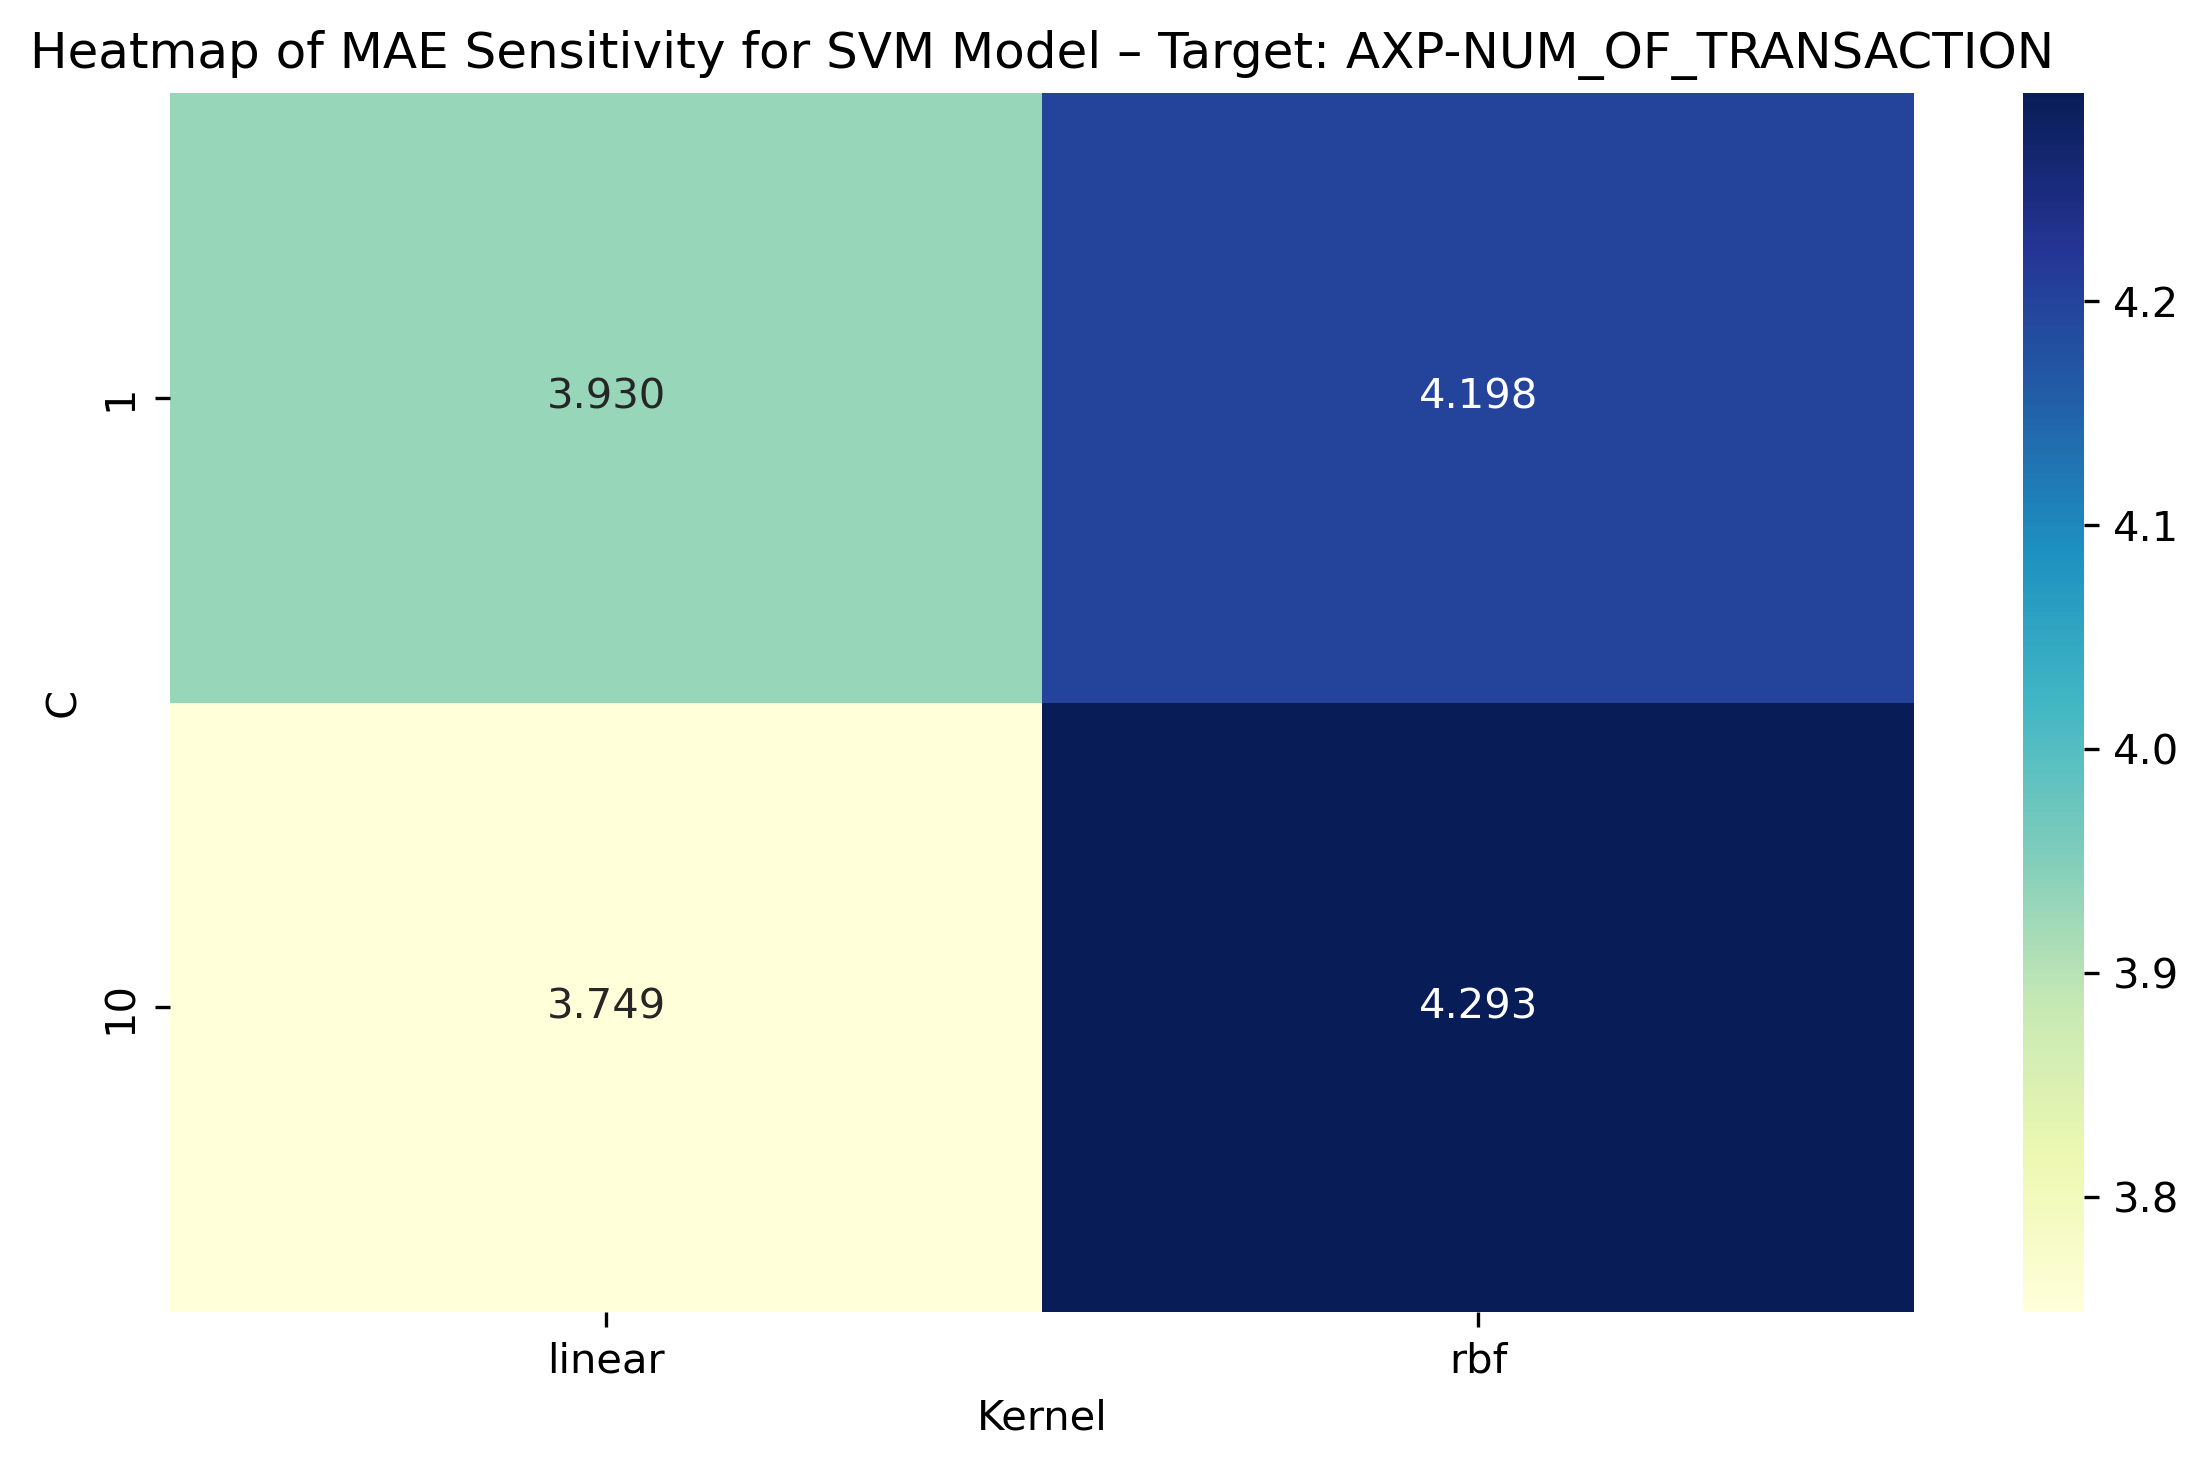
\includegraphics[width=\textwidth]{svm_mae_sensitivity_AXP-NUM_OF_TRANSACTION.png}
    \caption{SVM MAE – AXP}
    \label{fig:svm_mae_axp}
  \end{subfigure}
  \hfill
  \begin{subfigure}[b]{0.45\textwidth}
    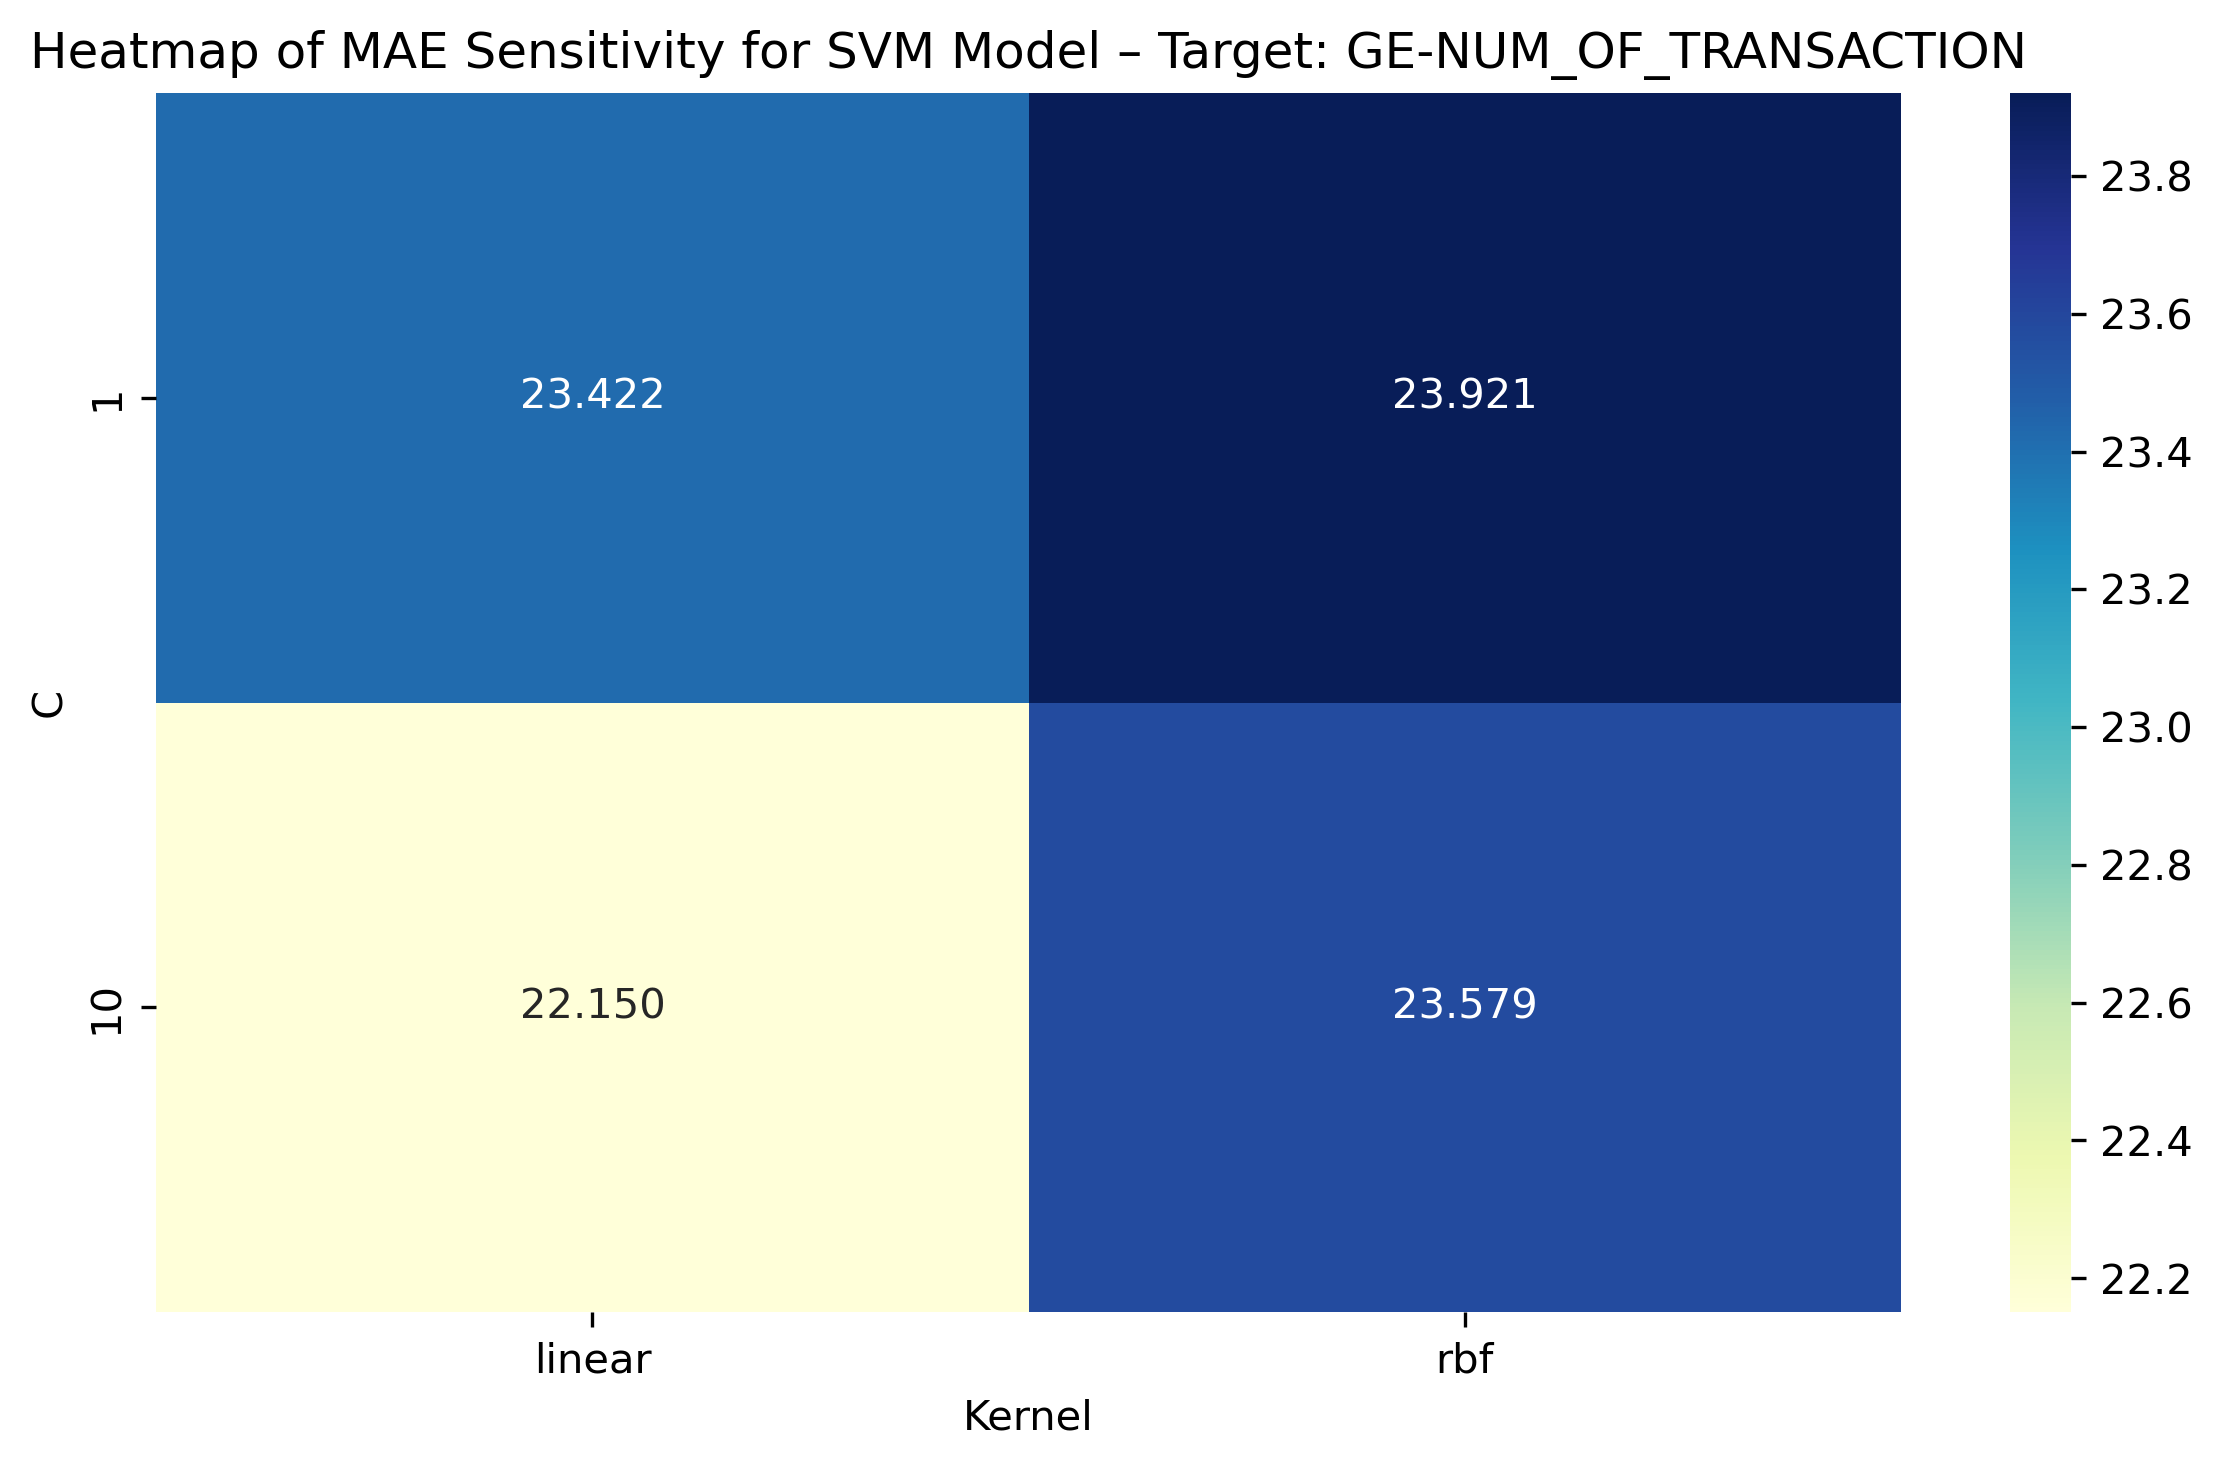
\includegraphics[width=\textwidth]{svm_mae_sensitivity_GE-NUM_OF_TRANSACTION.png}
    \caption{SVM MAE – GE}
    \label{fig:svm_mae_ge}
  \end{subfigure}
   \vspace{0.5cm}
\begin{subfigure}[b]{0.45\textwidth}
    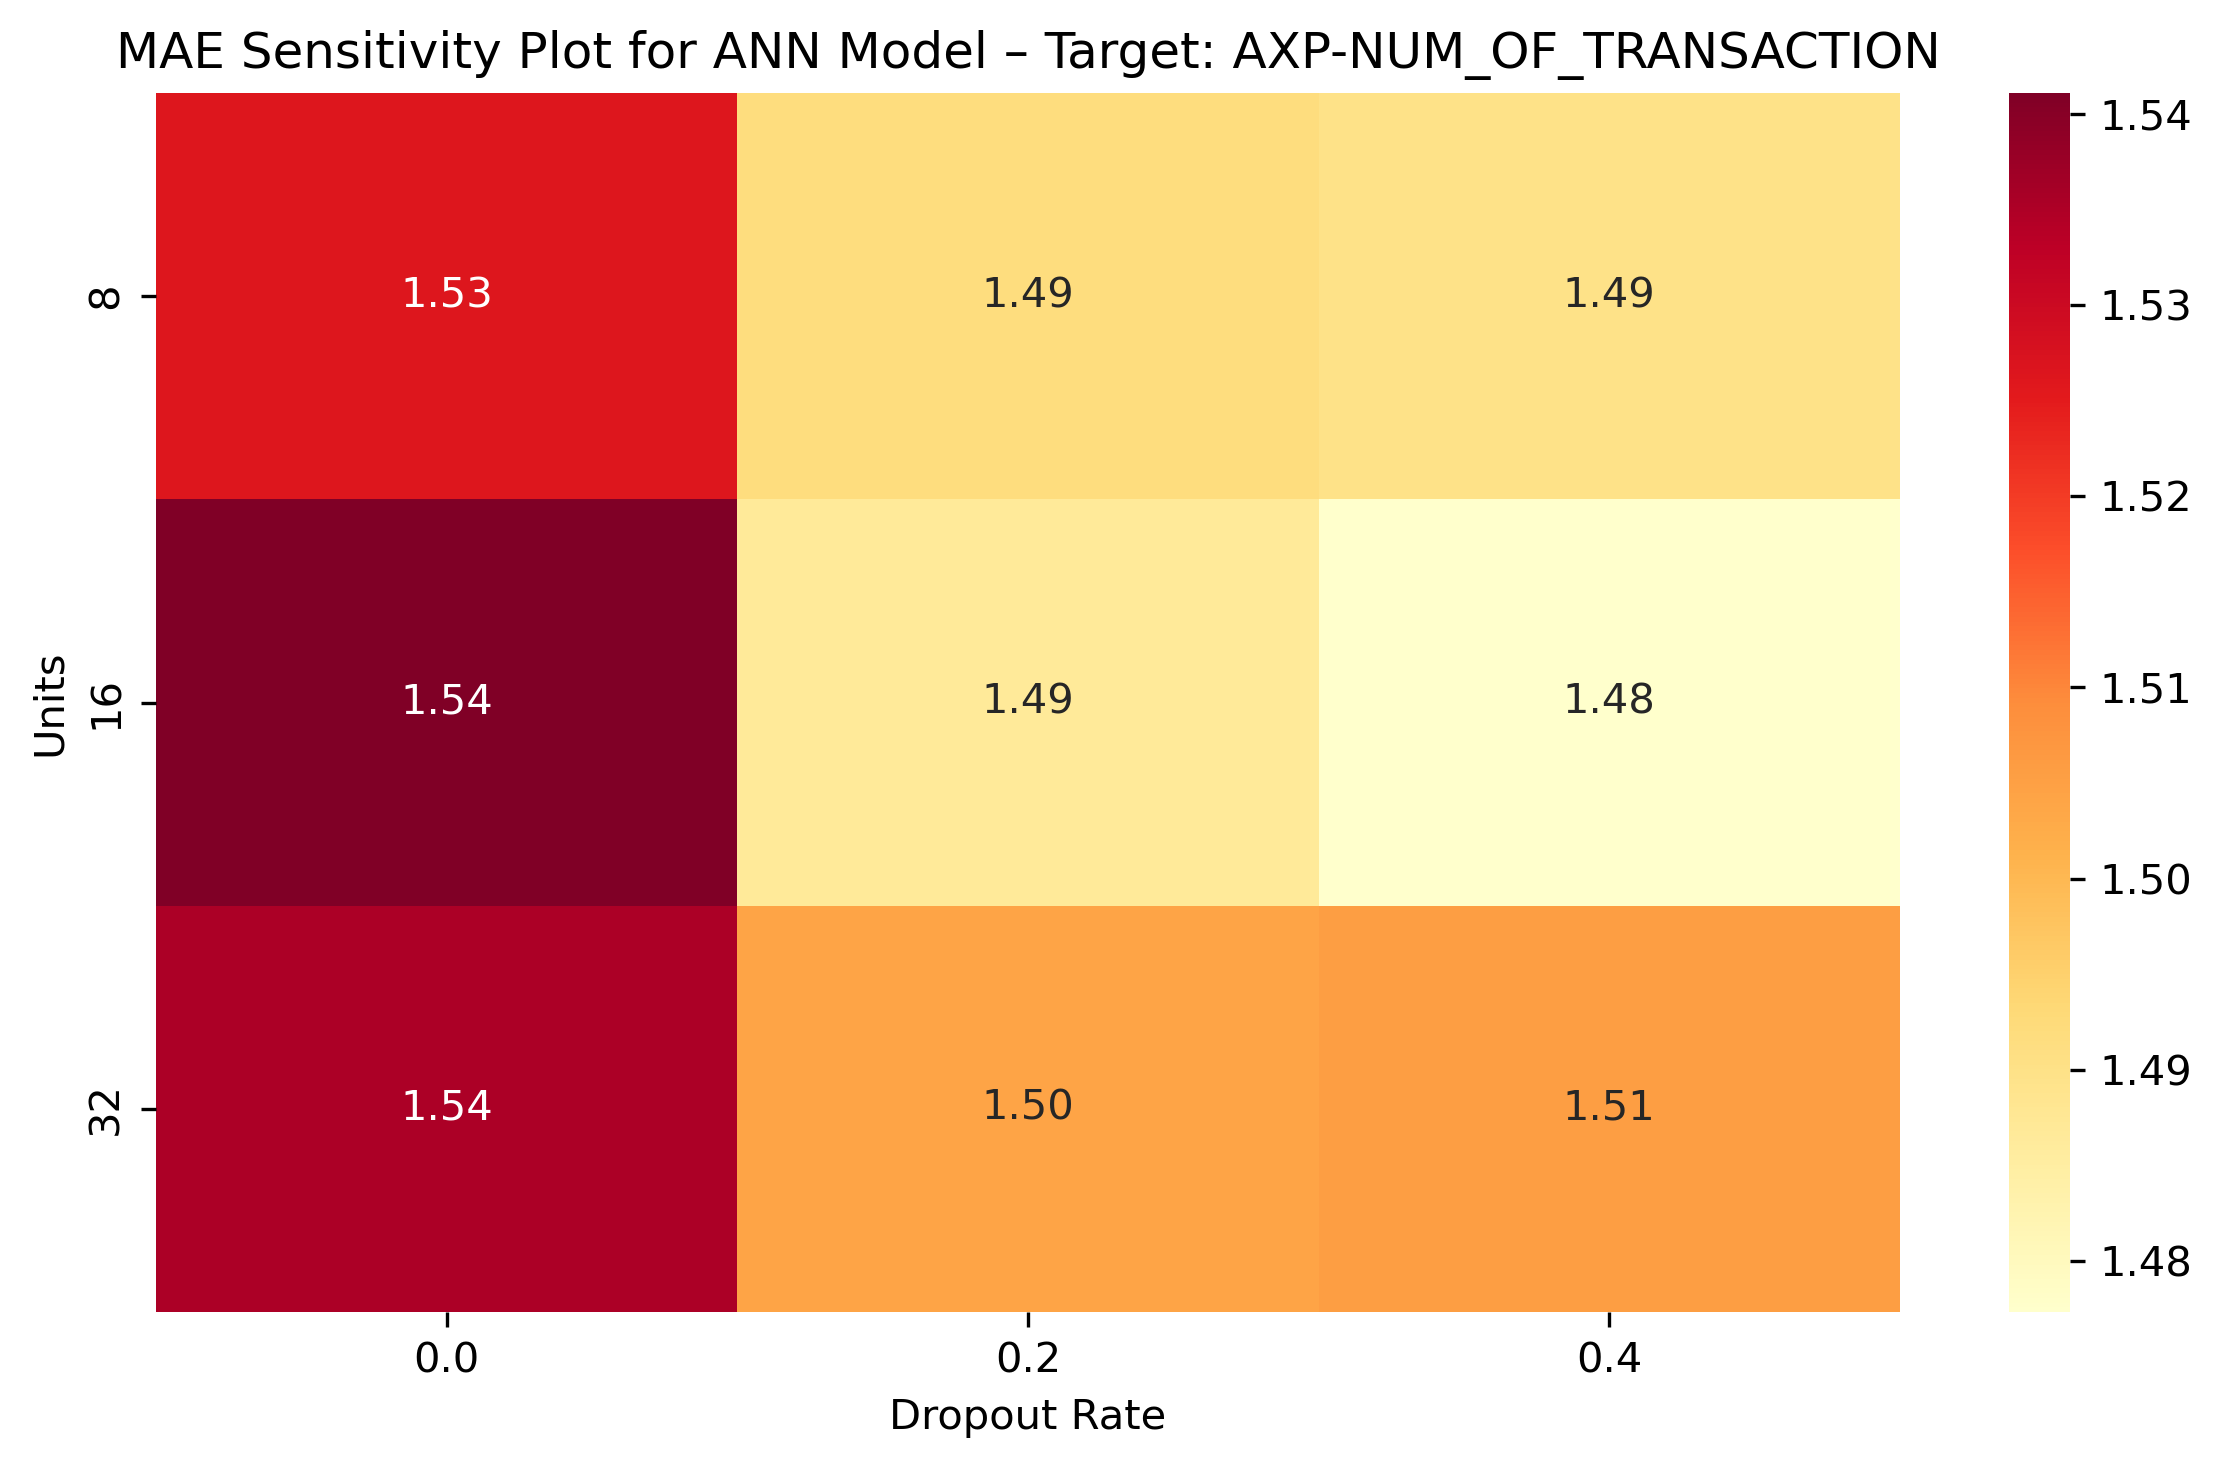
\includegraphics[width=\textwidth]{ann_mae_sensitivity_AXP-NUM_OF_TRANSACTION.png}
    \caption{ANN MAE – AXP}
    \label{fig:ann_mae_axp}
  \end{subfigure}
  \hfill
  \begin{subfigure}[b]{0.45\textwidth}
    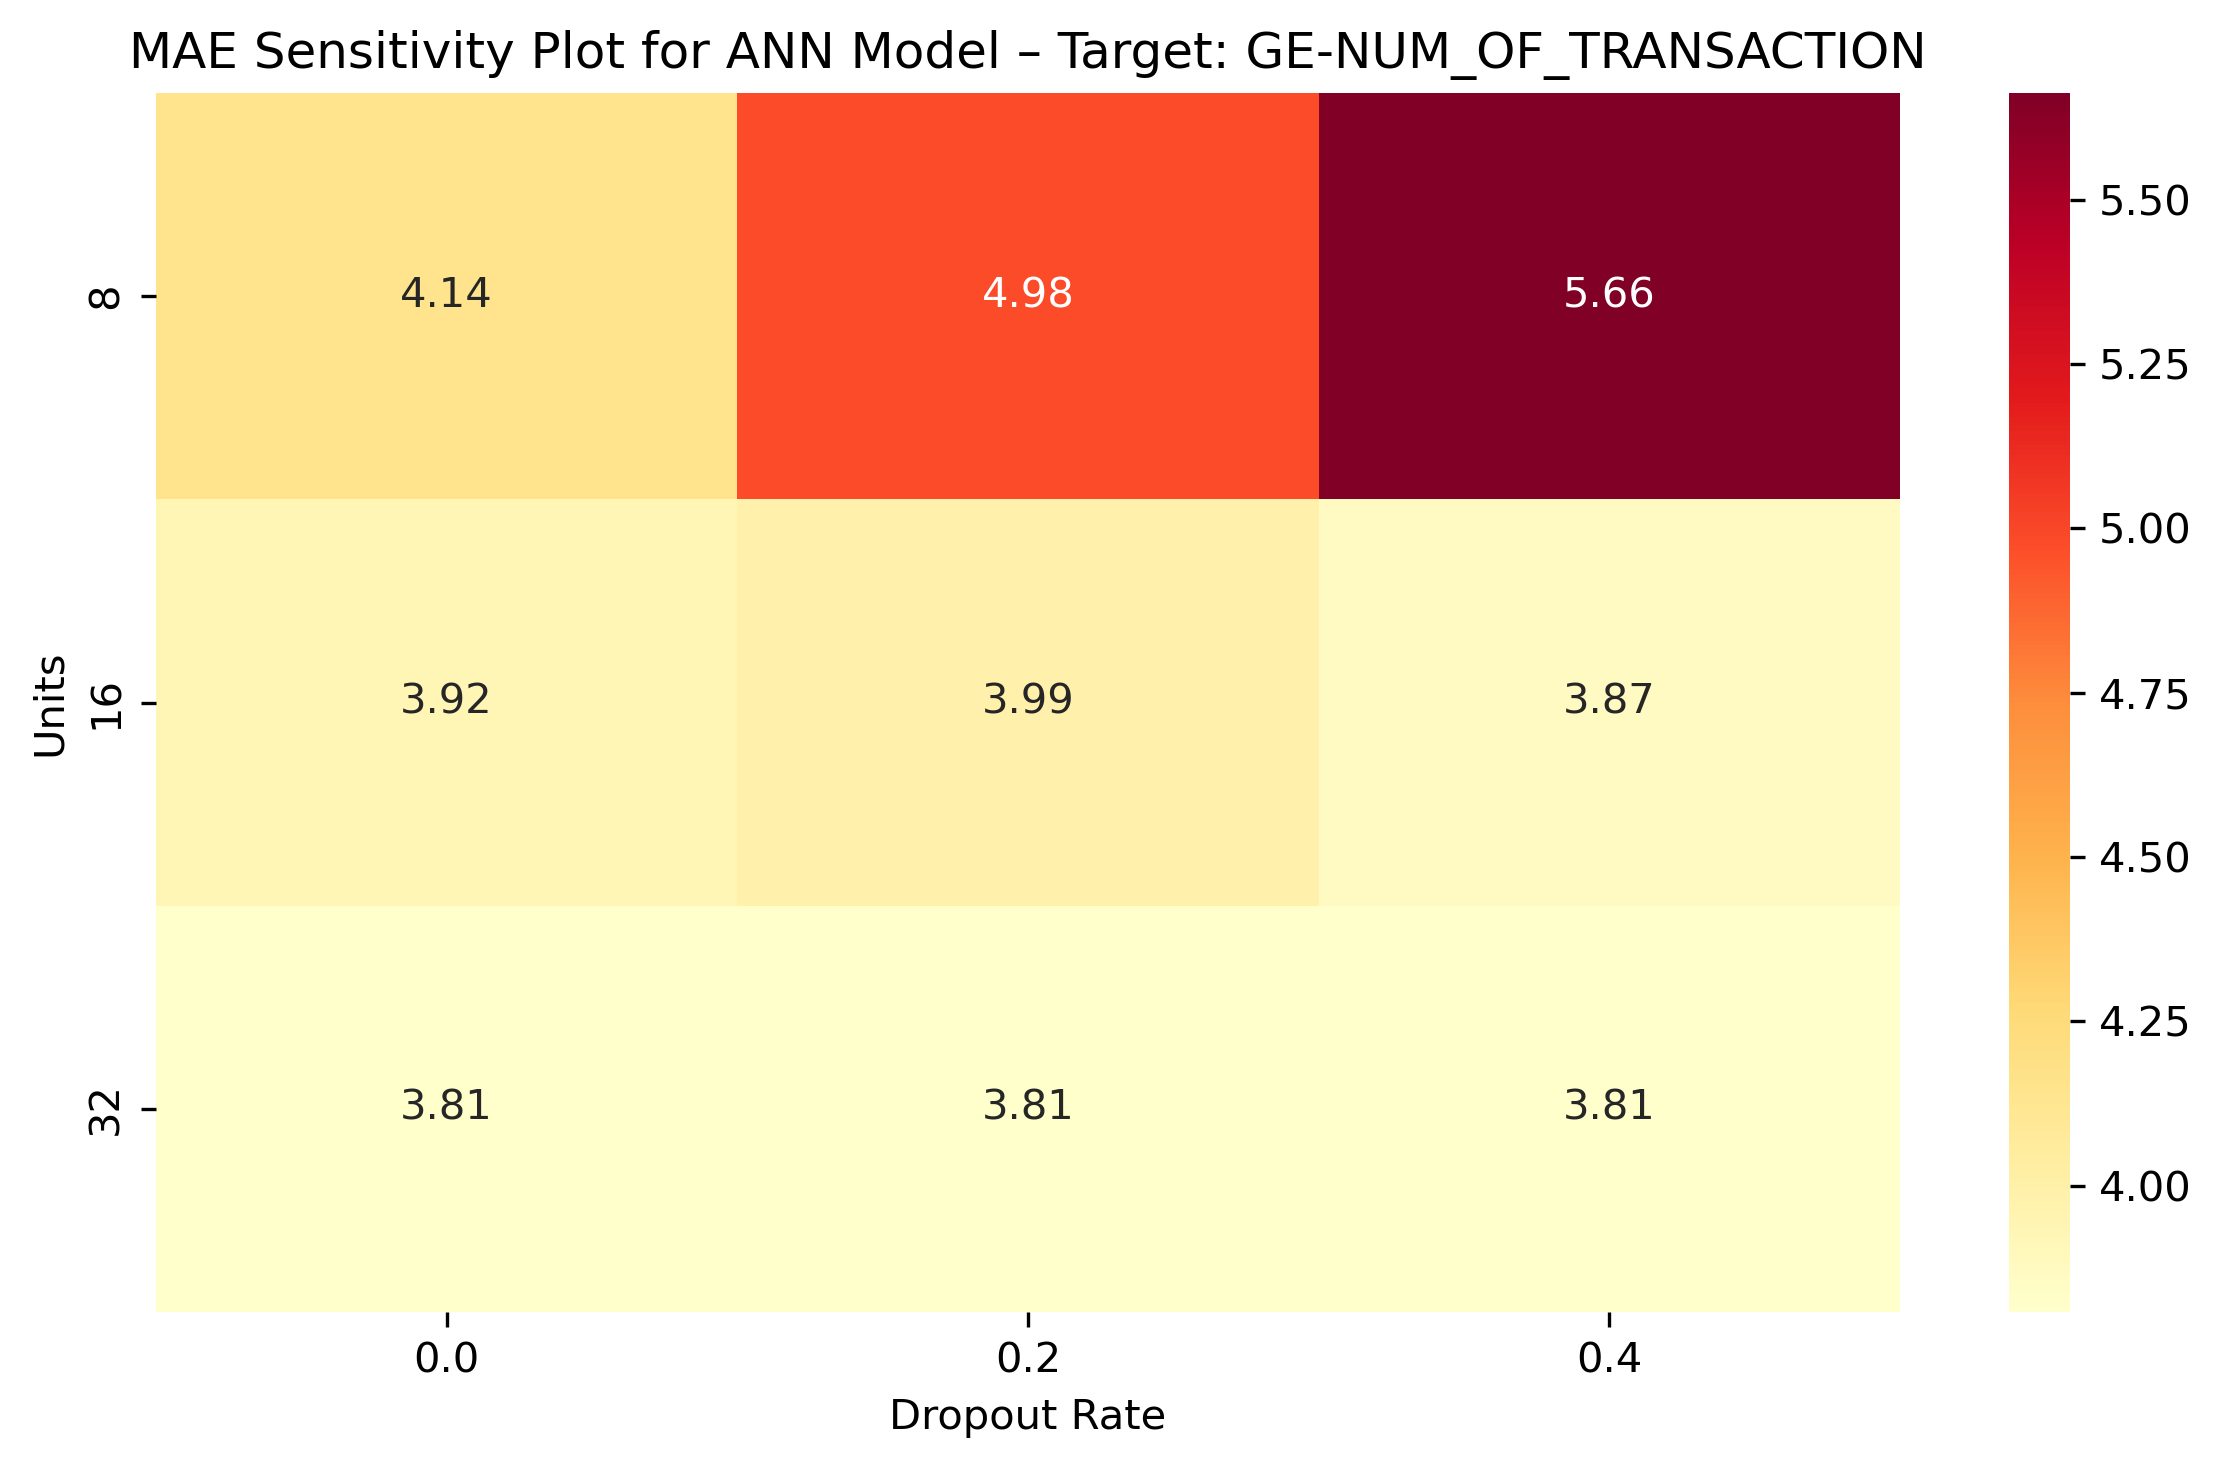
\includegraphics[width=\textwidth]{ann_mae_sensitivity_GE-NUM_OF_TRANSACTION.png}
    \caption{ANN MAE – GE}
    \label{fig:ann_mae_ge}
    \label{fig:ann_sensitivity_combined}
  \end{subfigure}
  \vspace{0.5cm}
\begin{subfigure}[b]{0.45\textwidth}
    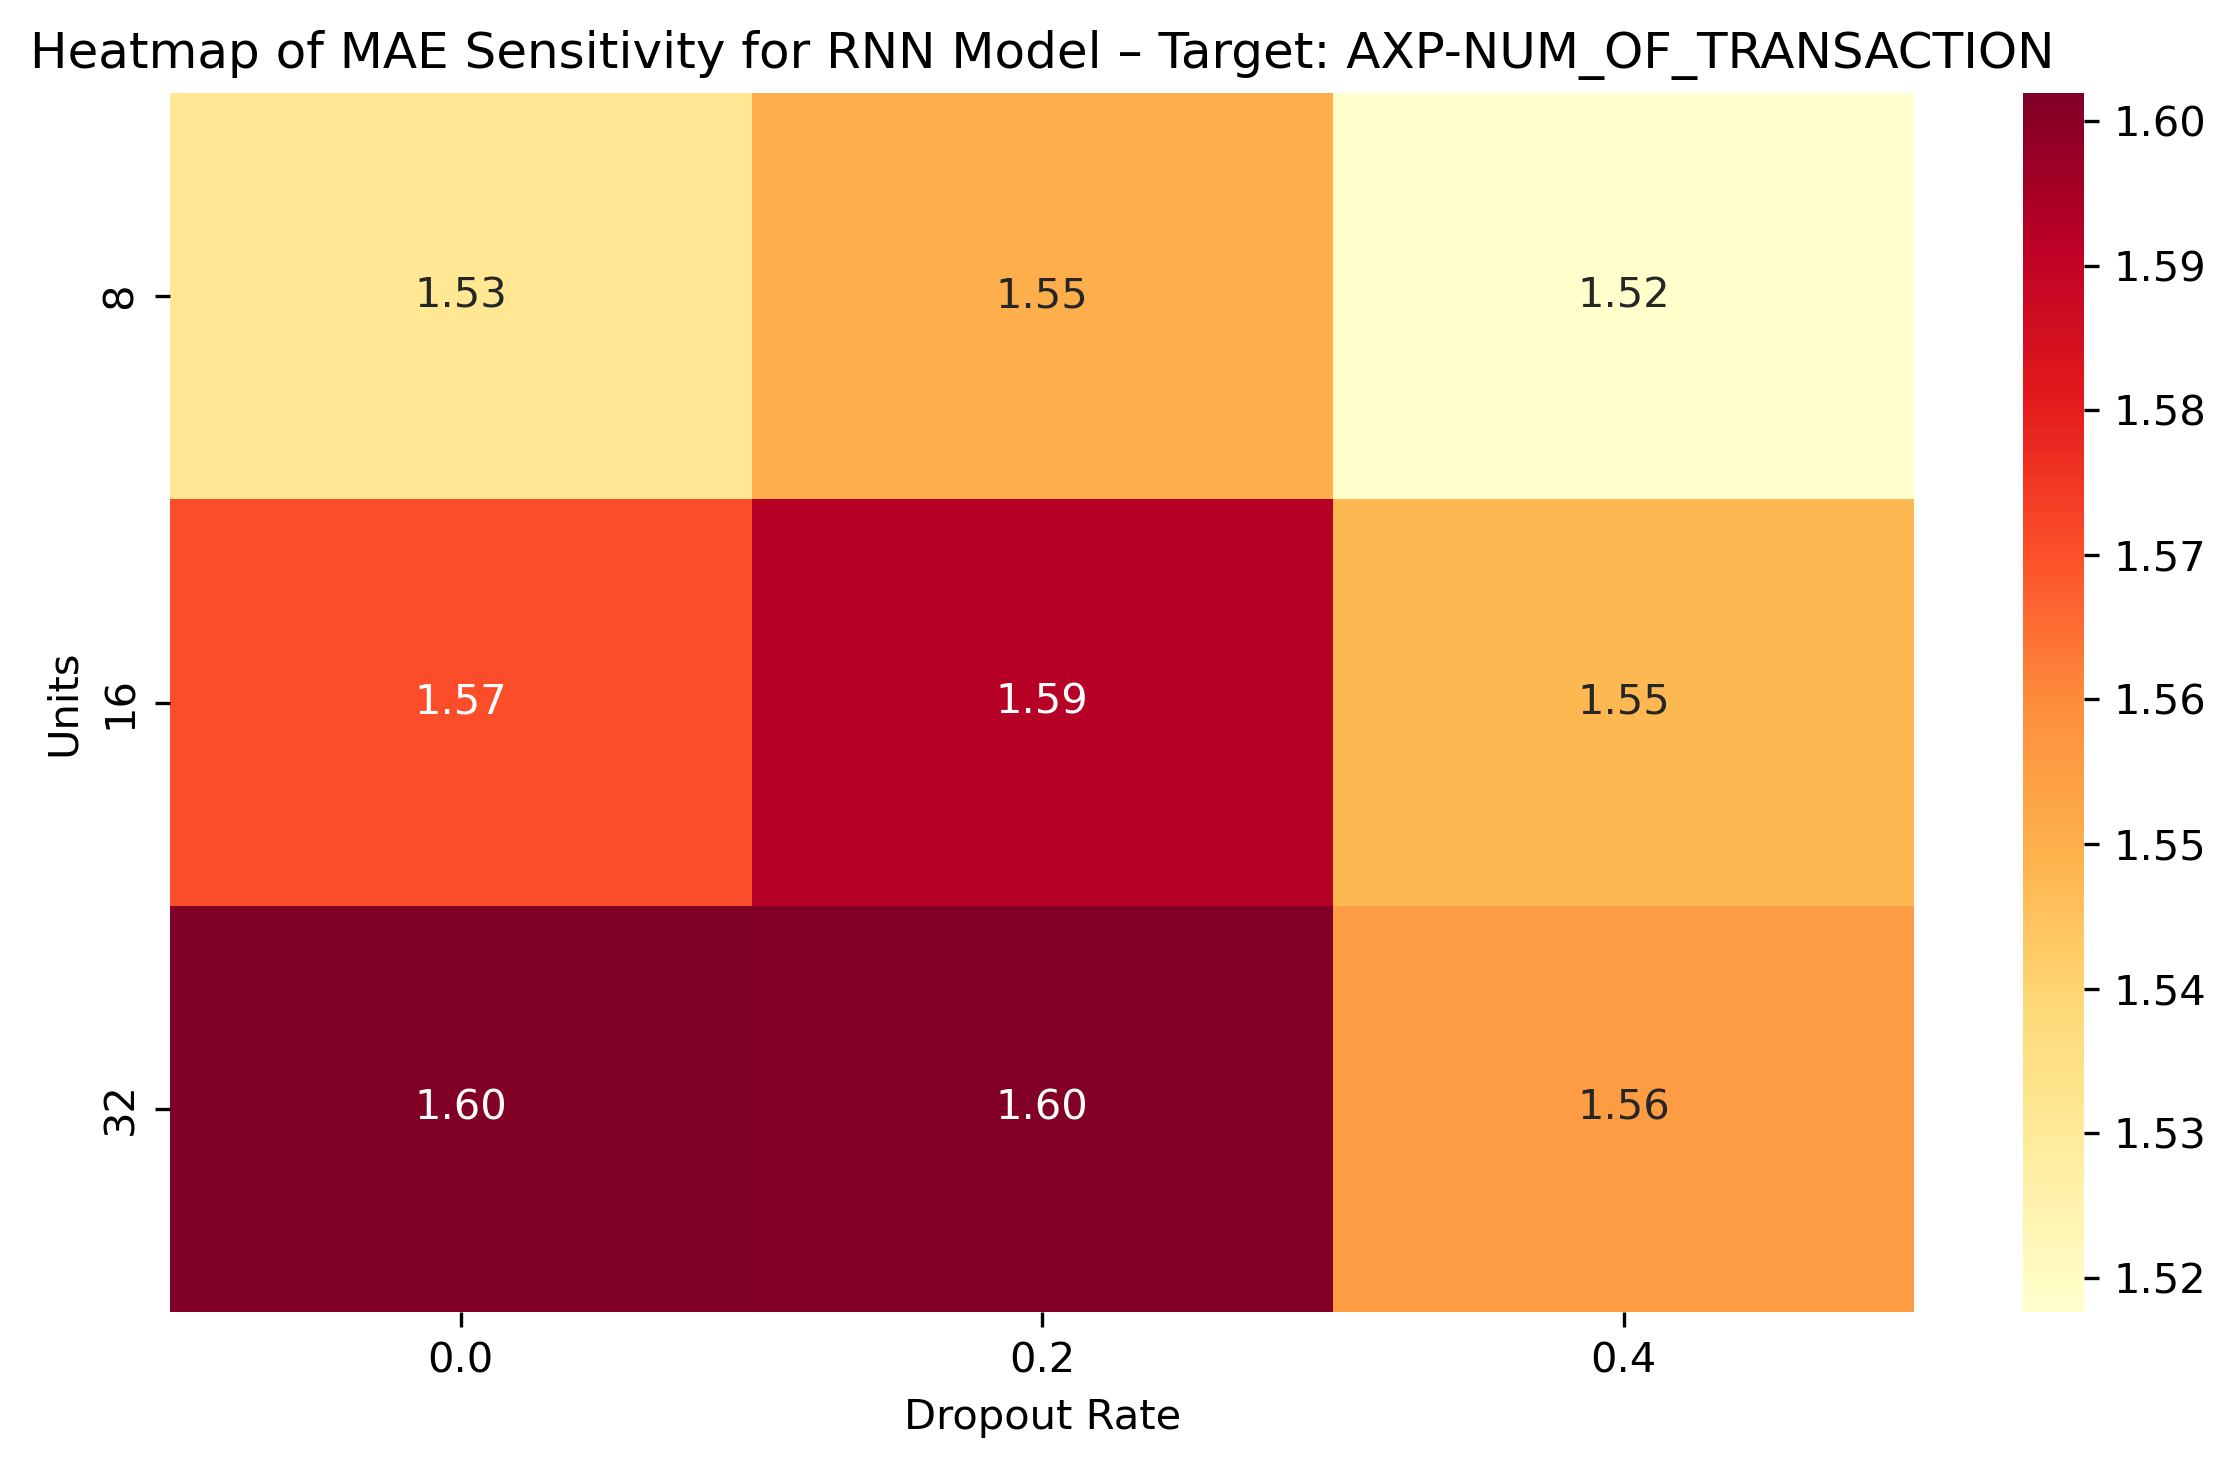
\includegraphics[width=\textwidth]{rnn_mae_sensitivity_AXP-NUM_OF_TRANSACTION.png}
    \caption{RNN MAE – AXP}
    \label{fig:rnn_mae_axp}
  \end{subfigure}
  \hfill
  \begin{subfigure}[b]{0.45\textwidth}
    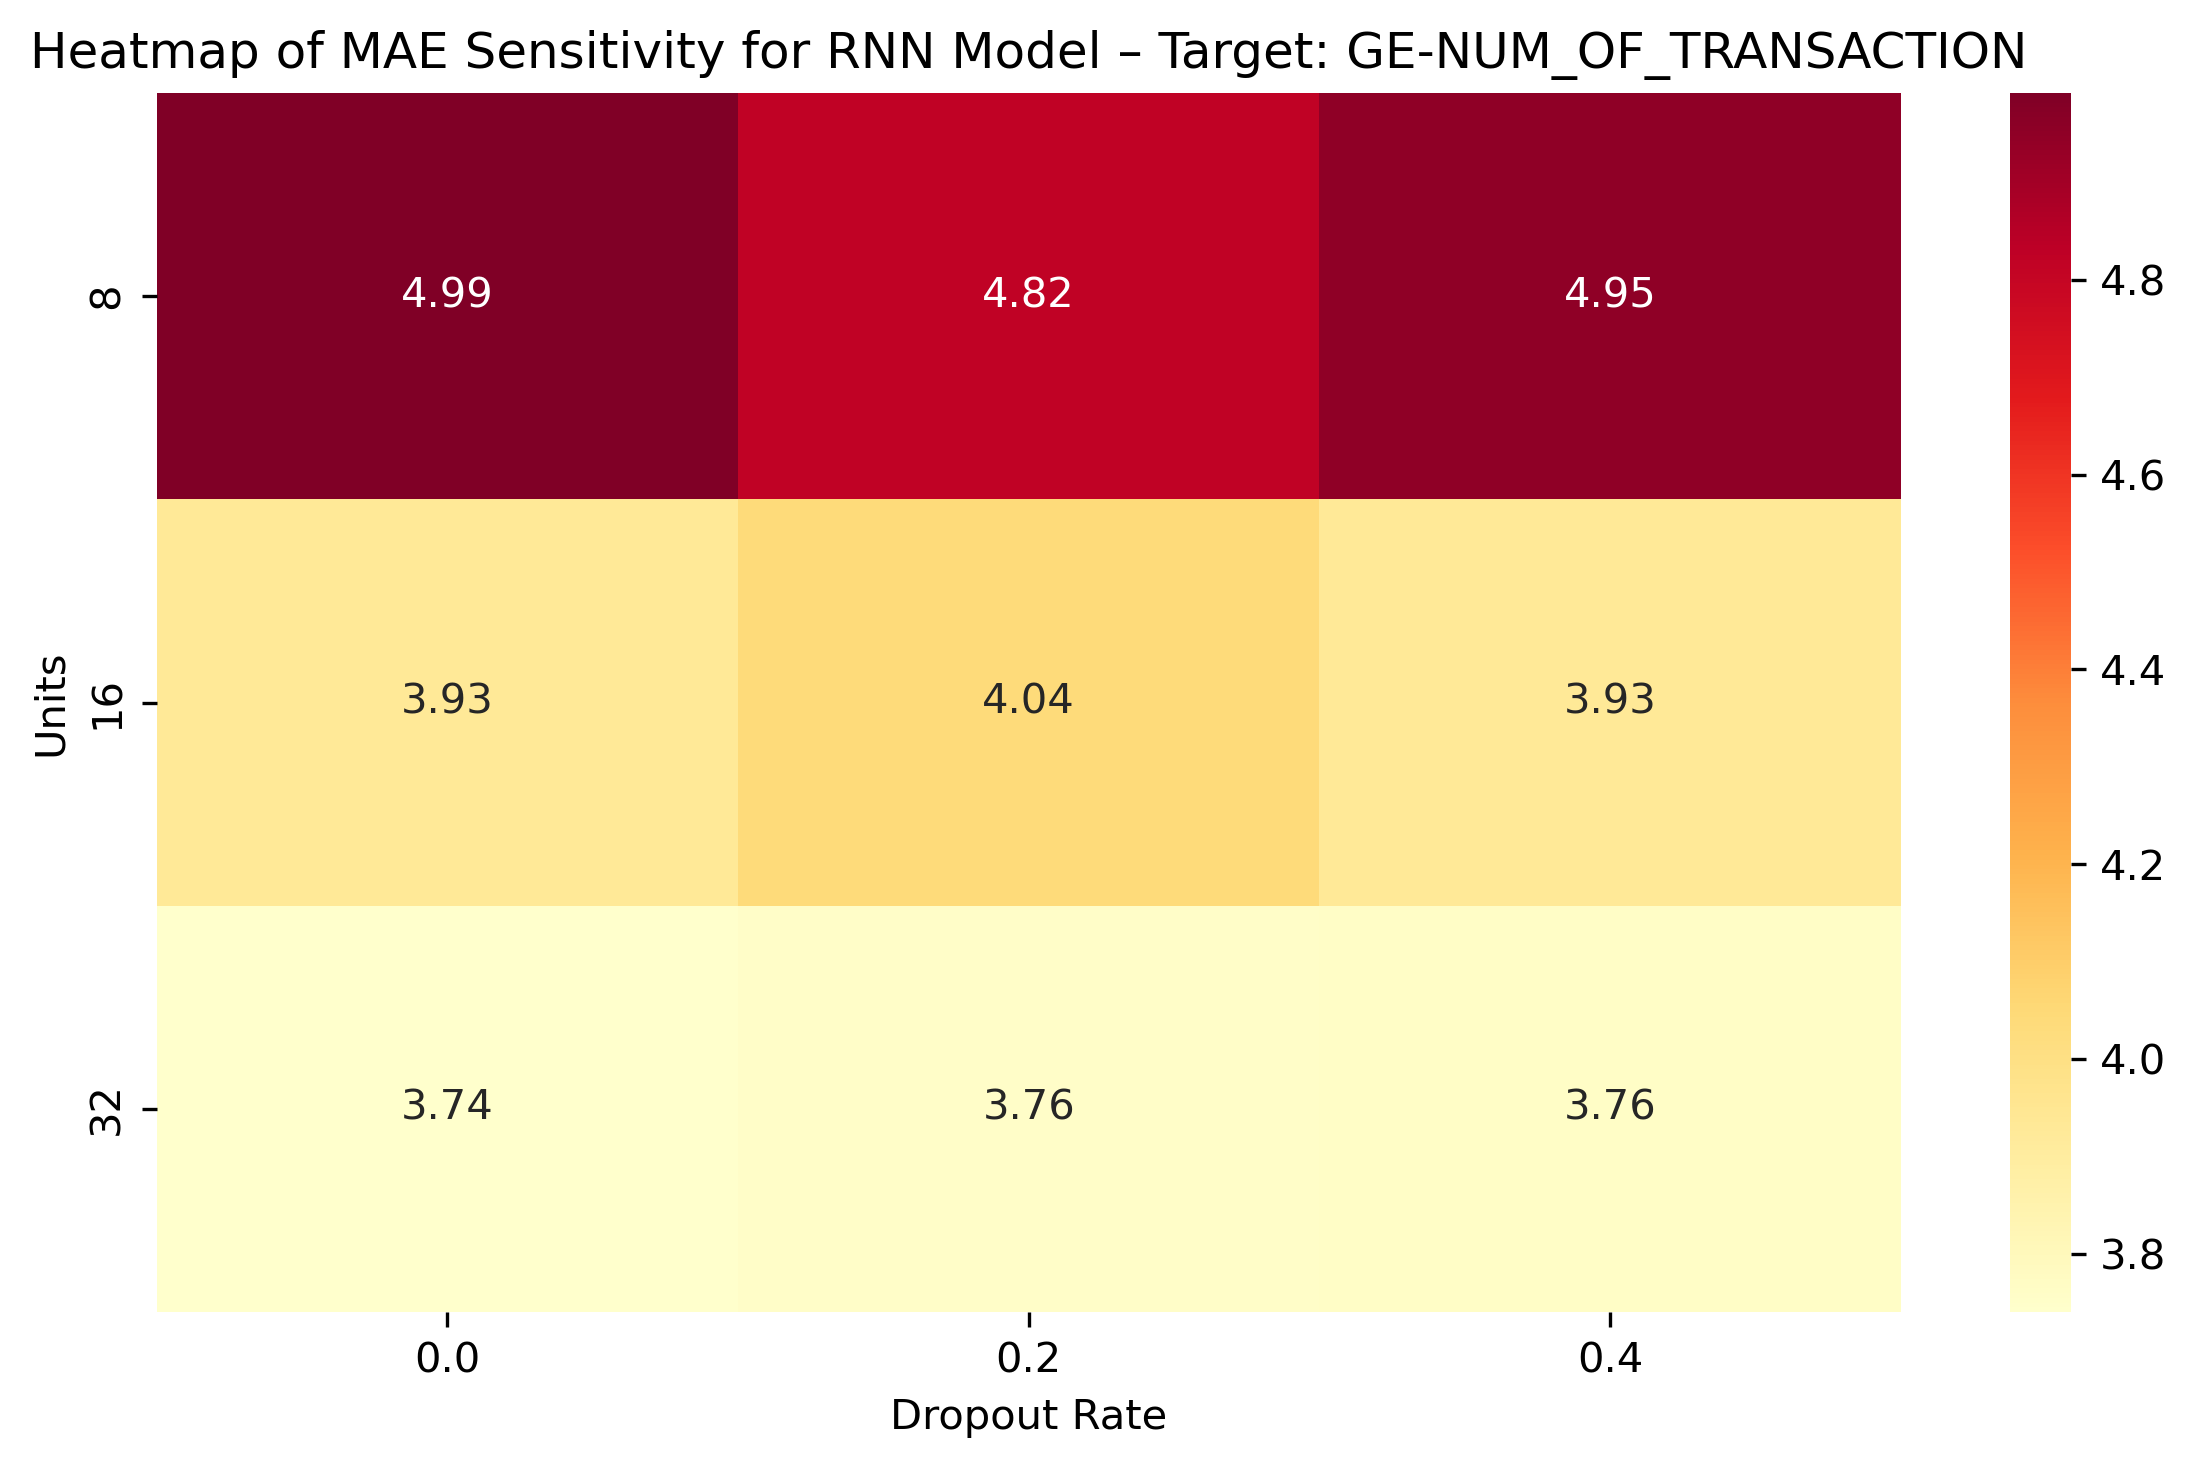
\includegraphics[width=\textwidth]{rnn_mae_sensitivity_GE-NUM_OF_TRANSACTION.png}
    \caption{RNN MAE – GE}
    \label{fig:rnn_mae_ge}
     \label{fig:rnn_sensitivity_combined}
  \end{subfigure}
  \vspace{0.5cm}
  \begin{subfigure}[b]{0.45\textwidth}
    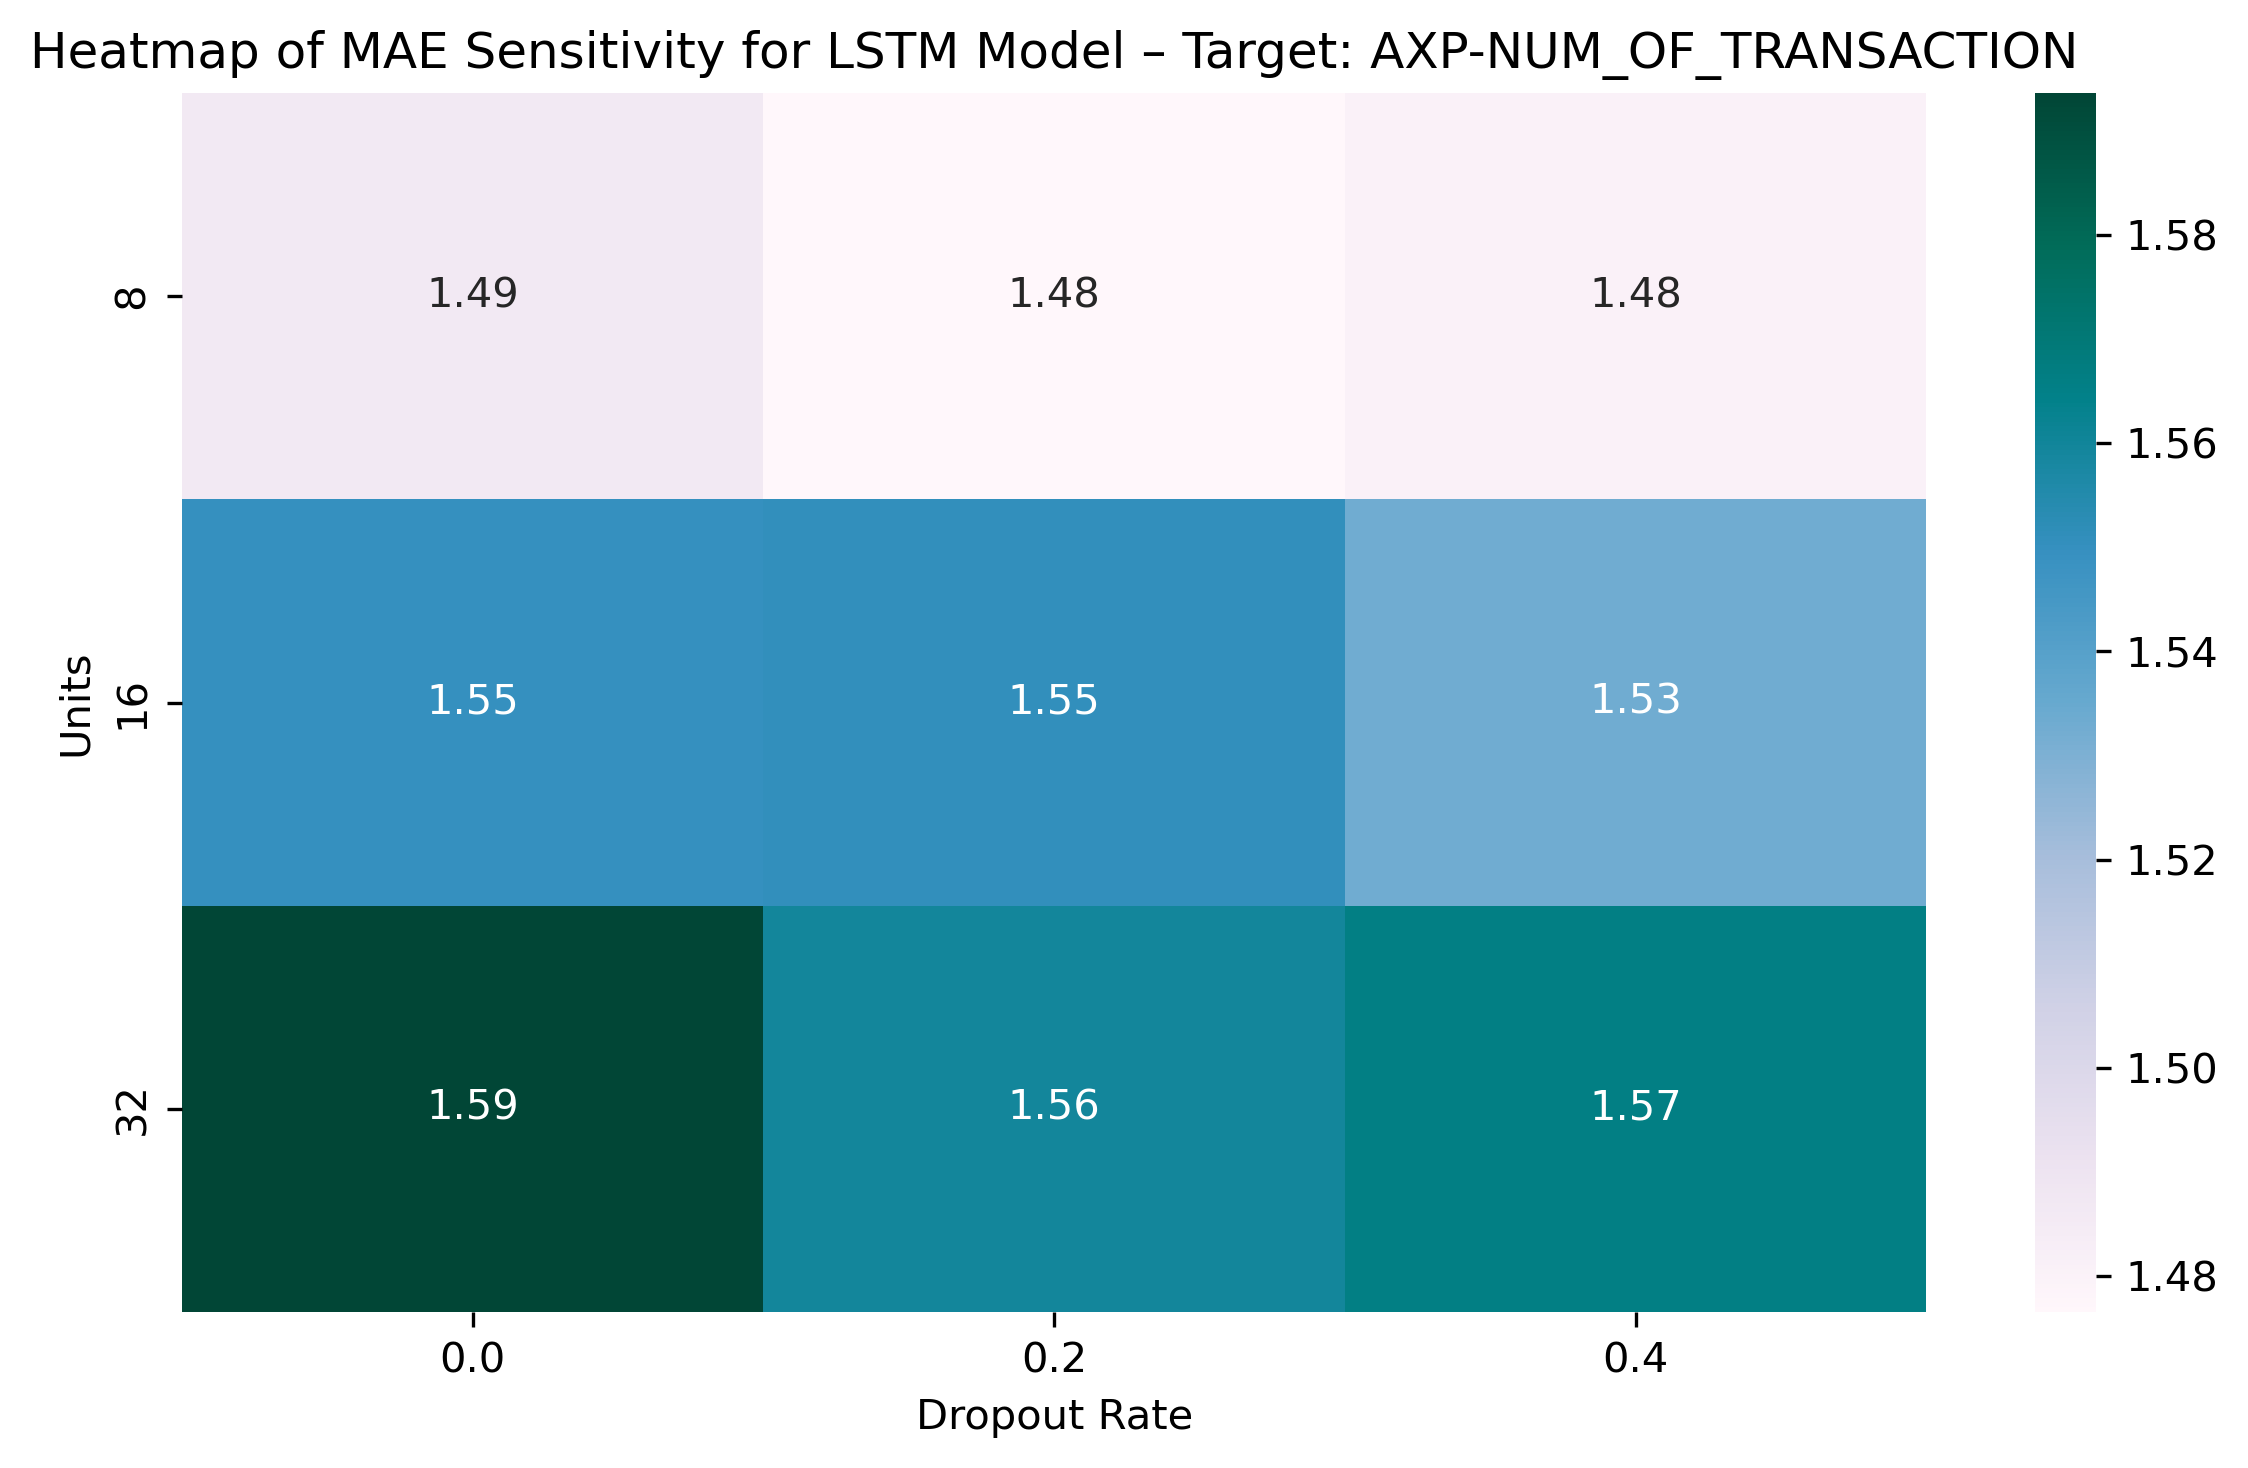
\includegraphics[width=\textwidth]{lstm_mae_sensitivity_AXP-NUM_OF_TRANSACTION.png}
    \caption{LSTM MAE – AXP}
    \label{fig:lstm_mae_axp}
  \end{subfigure}
  \hfill
  \begin{subfigure}[b]{0.45\textwidth}
    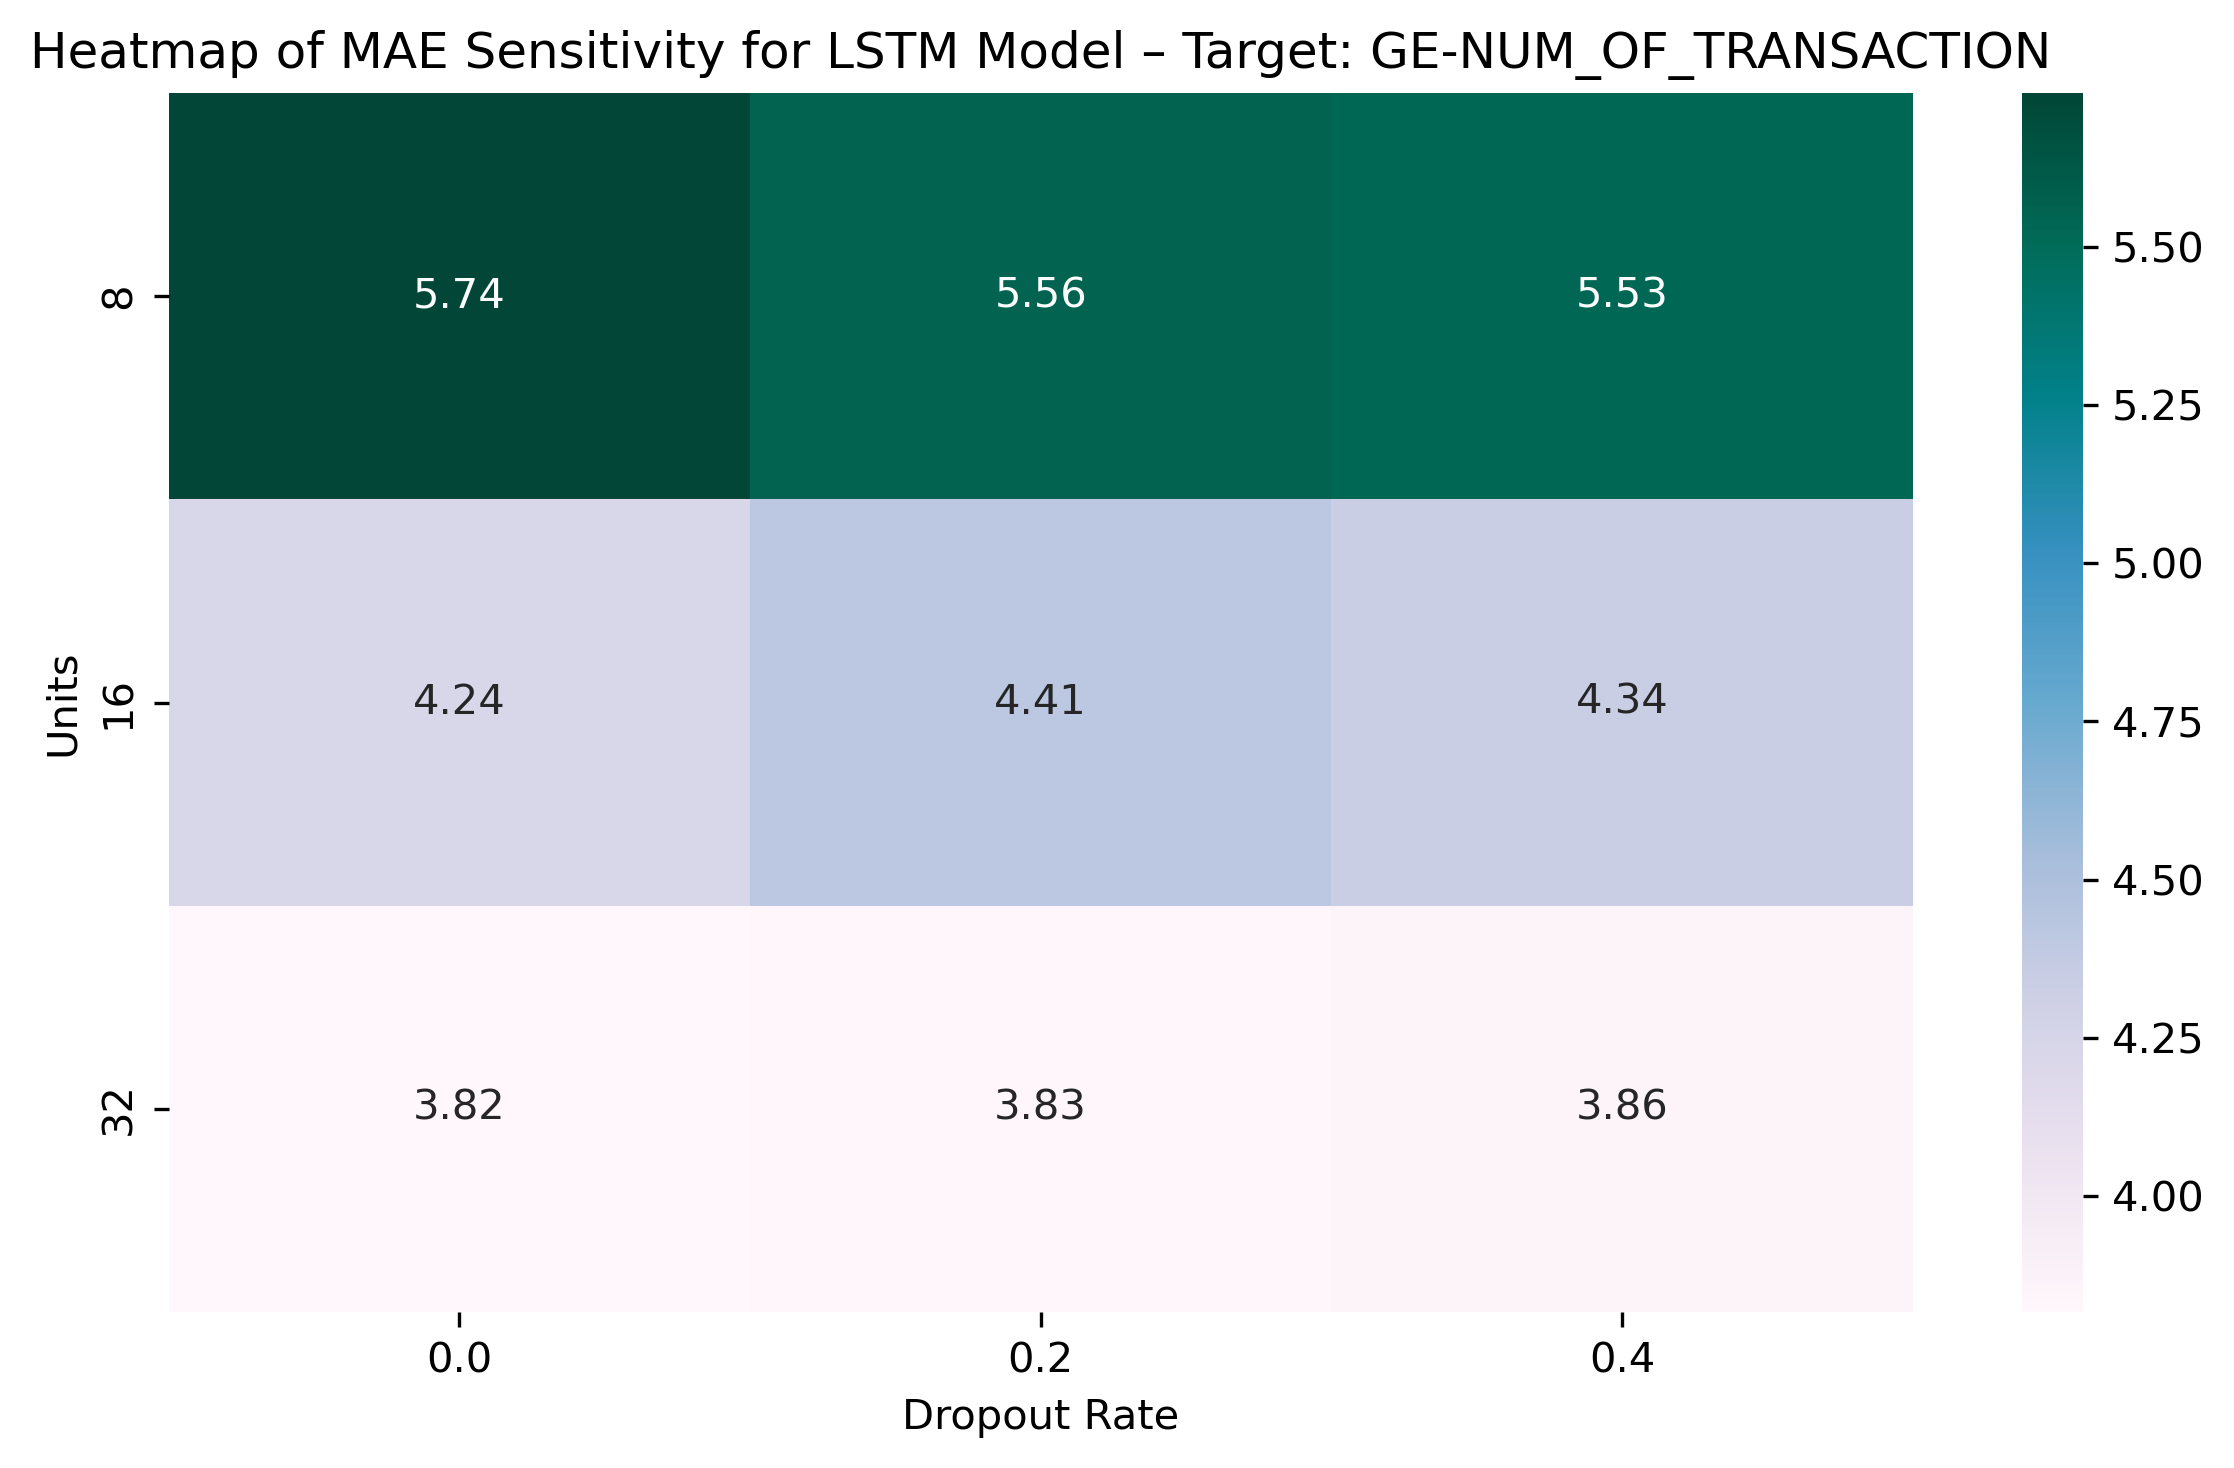
\includegraphics[width=\textwidth]{lstm_mae_sensitivity_GE-NUM_OF_TRANSACTION.png}
    \caption{LSTM MAE – GE}
    \label{fig:lstm_mae_ge}
     \label{fig:lstm_sensitivity_combined}
  \end{subfigure}
  \caption{Heatmap plots of MAE sensitivity for SVM, ANN, RNN, and LSTM models predicting number of transactions for AXP and GE.}
  \label{fig:svm_sensitivity_combined}
\end{figure}\\
\section{Conclusion}%\label{conclusion}
Across the evaluated machine learning models, SVM achieved the lowest test MAE across the target variables, indicating strong generalization and robust performance under different data conditions. The small relative error between predicted and actual values further confirms its prediction accuracy and consistency. These results suggest that SVM is well suited for structured, lower‑dimensional datasets, whereas LSTM may be more appropriate for modeling complex or sequential patterns.% Additionally, the small generalization gaps among the models indicate minimal overfitting, while future studies could explore ensemble learning methods on larger datasets to further improve performance. 
%\newpage
\begin{thebibliography}{99}
\bibitem[Alomair(2024)]{Alomair : 2024}
 Alomair, G., 2024. {\it Predictive performance of count regression models versus machine learning techniques: A comparative analysis using an automobile insurance claims frequency dataset}. PloS one, 19 (12):e0314975.

\bibitem[Al-Osh and  Alzaid (1987)]{Al-Osh and  Alzaid: 1987}
 Al-Osh, M. A., and A. A. Alzaid. 1987., {\it First-order integer-valued autoregressive (INAR(1)) process}. Journal of Time Series Analysis 8 (3):261–75.

\bibitem[Hewamalage( 2021)]{Hewamalage : 2021}
 Hewamalage, H., Bergmeir, C. and Bandara, K., 2021. {\it Recurrent neural networks for time series forecasting: Current status and future directions}. International Journal of Forecasting, 37 (1):388-427.

\bibitem[Ilemobayo(2024)]{Ilemobayo : 2024}
 Ilemobayo, J. A., Durodola, O., Alade, O., Awotunde, O.J., Olanrewaju, A.T., Falana, O., Ogungbire, A., Osinuga, A., Ogunbiyi, D., Ifeanyi, A. and Odezuligbo, I.E., 2024. {\it Hyperparameter tuning in machine learning: A comprehensive review}. Journal of Engineering Research and Reports 26 (6):388-395.

\bibitem[Lim (2021)]{Lim : 2021}
 Lim, B. and Zohren, S., 2021. {\it Time-series forecasting with deep learning: a survey}. Philosophical Transactions of the Royal Society A 379(2194):20200209.

\bibitem[McKenzie(1986)]{McKenzie: 1986}
 McKenzie, E. 1986., {\it Autoregressive moving-average processes with negative binomial and geometric marginal distributions.} Advances in Applied Probability 18 (3):679–705. 

\bibitem[Nyholm(2003)]{Nyholm : 2003}
 Nyholm, K. 2003., {\it Inferring the private information content of trades: A regime-switching approach}. Journal of Applied Econometrics 18 (4):457–70.

\bibitem[Pedeli and  Karlis (2013)]{Pedeli  and Karlis: 2013}
l  Pedeli, X., and D. Karlis. 2011., {\it  A bivariate INAR(1) process with application}. Statistical Modelling 11 (4):325–49.

\bibitem[Rathod(2021)]{Rathod : 2021}
Rathod, S., Yerram, S., Arya, P., Katti, G., Rani, J., Padmakumari, A.P., Somasekhar, N., Padmavathi, C., Ondrasek, G., Amudan, S. and Malathi, S., 2021. {\it Climate-based modeling and prediction of rice gall midge populations using count time series and machine learning approaches}. Agronomy, 12 (1):22.

\bibitem[Schweer(2014)]{Schweer : 2014}
 Schweer, S., and C. H. Weiß. 2014. {\it Compound Poisson INAR(1) processes: Stochastic properties and testing for overdispersion}. Computational Statistics \& Data Analysis 77:267–84.
\end{thebibliography}
\end{document}